\section{Evaluation}

Recently, Haehn et al. discussed requirements for interactive proofreading software and evaluated three different existing tools on connectomics data \cite{haehn_dojo_2014}. The authors performed a non-expert user study and stated that their software Dojo provides better results than other tools due to a minimalistic user interface and sophisticated 3D volume rendering. We use their findings as baseline for the evaluation of our method and compare \textit{fully automatic proofreading} versus \textit{user-guided proofreading} versus \textit{interactive proofreading}. For comparison, we use the same data as Haehn et al. which is as well as the user generated proofreading results, publicly available. The data is part of the ISBI 2013 challenge dataset (1024x1024x100 pixels) which was acquired using a serial section scanning electron microscope (ssSEM) with a resolution of 6x6x30nm/pixel. Haehn et al. perform their user study on the most representative sub-volume (400x400x10 pixels) in terms of distribution of object size. For optimal comparison, we use exactly the same data.

Each method is compared against the available manually labeled ground truth of the data for similarity and is scored using the variation of information (VI) metric. VI is a measure of the distance between two clusterings, closely related to mutual information, but lower being better.

Since our classifiers are trained on 2D images, we perform all evaluations on slices rather than image stacks. We choose the best performing network variation as well as the parameters based on experiments using the last five slices of our original training and testing data (\ref{sec:method}). 


\textbf{Fully automatic proofreading.} During training, we defined parameters for our split and merge classifiers including thresholds for automatic correction of these. To evaluate automatic proofreading, we use both classifiers in a greedy fashion and choose the split and merge errors with the highest scores for automatic correction. First, we performed merge error correction with $\max(1-p)$, followed by split error correction using a probability threshold $p_t=.95$. The total time for the correction was 17 minutes (merge error correction 15min, split error correction 2min). The average VI improvement in comparison to the ground truth was $.022$ ($.013$ for only split error correction).

\textbf{User-guided proofreading.} For the evaluation of user-guided proofreading, we simulate user feedback during our automatic correction from above by comparing the resulting segmentation before and after each performed correction. Since users are not perfect, we also introduce an error rate which simulates falsely specified user feedback. This error rate defines if we accept a good split or reject it as well as accept a bad split or reject such, based on direct comparison with the ground truth using a scoring metric. Assuming a perfect user with an error rate of 0, the average VI improvement in comparison to the ground truth was $.11$.

\textbf{Interactive proofreading.} We use the published results from Haehn et al. to compare our results against fully interactive proofreading using their software Dojo. Since the performance between participants of Haehn's user study shows large differences, we decided to choose the best performing user (VI improvement $.0598$) as well as the average performance among all users (VI improvement $-.012$) as our baseline.

\begin{figure}[t]
\centering
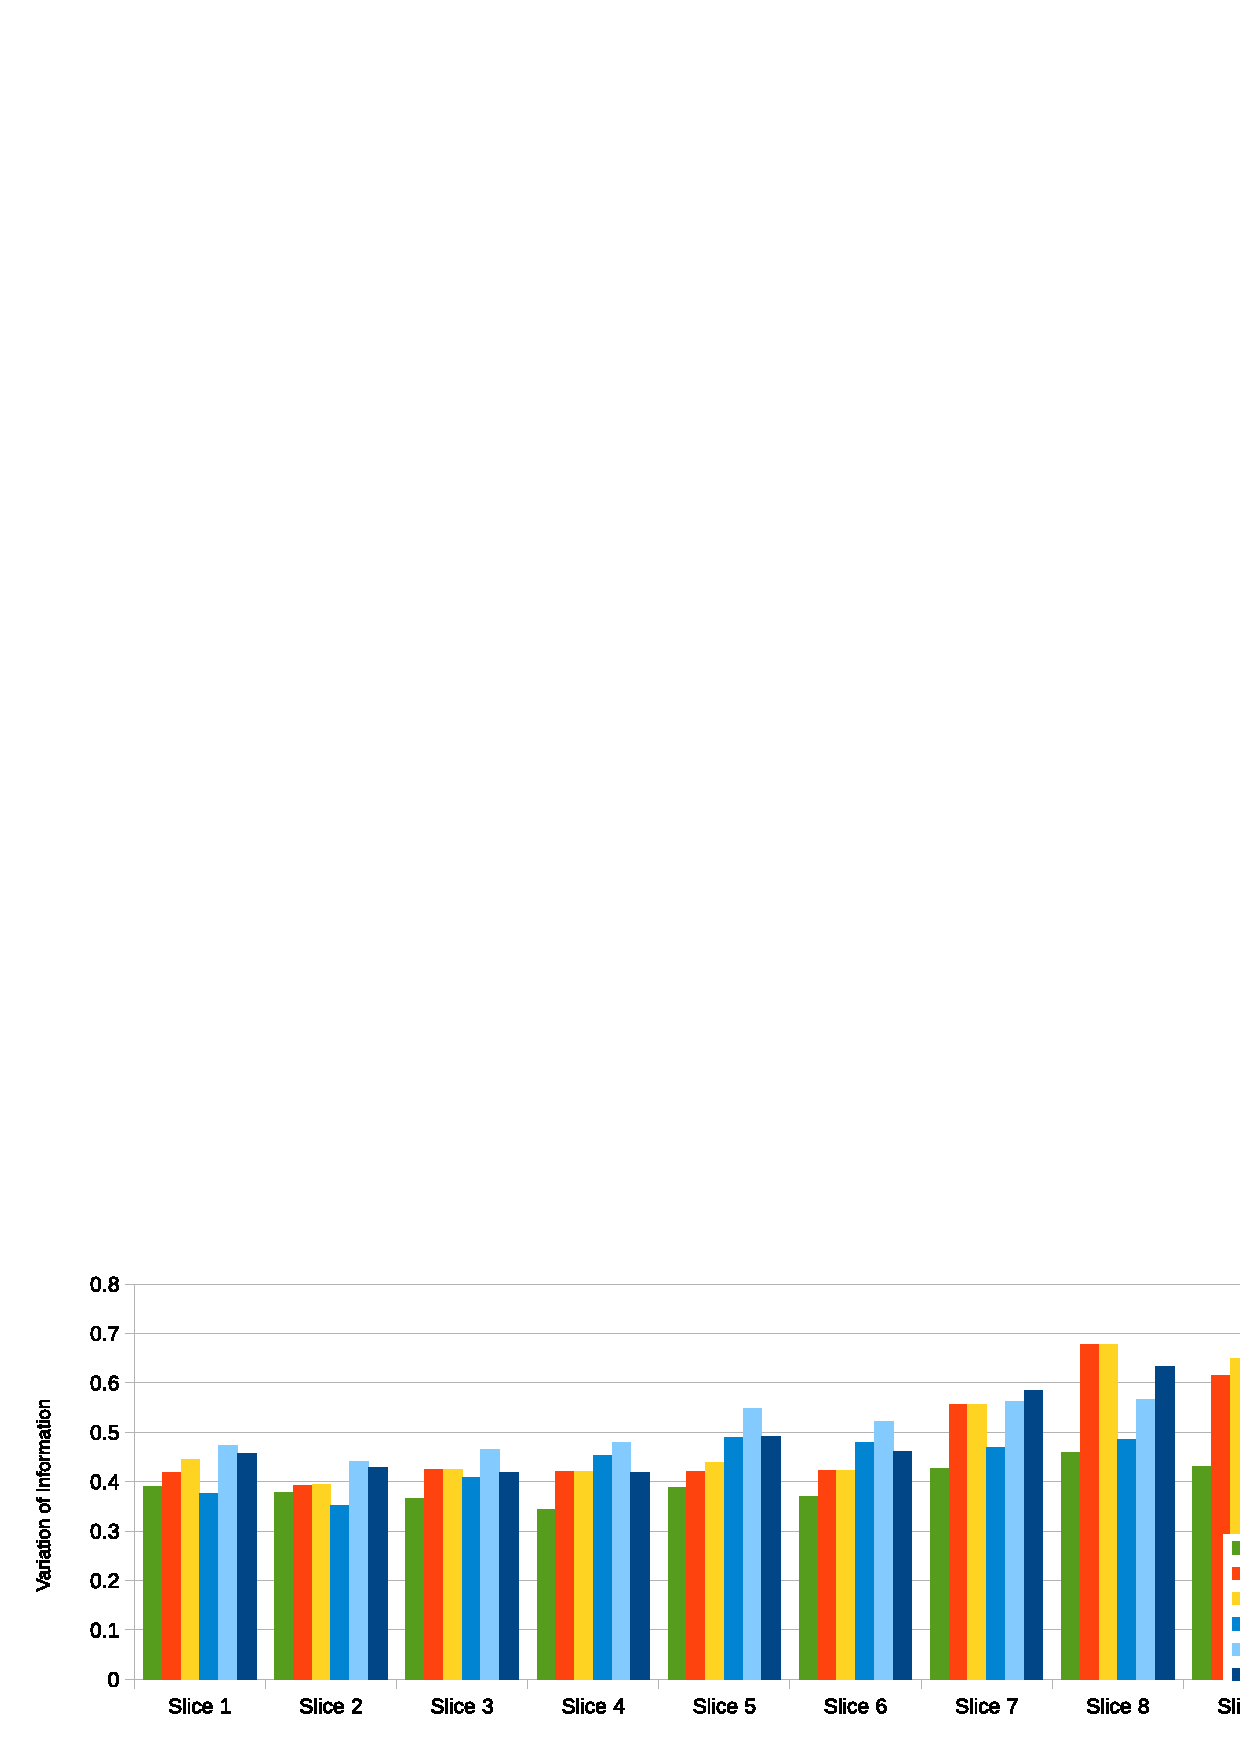
\includegraphics[scale=.45]{gfx/results.pdf}
\caption{We compare user-guided (error rate .0) and automatic (full+just splits) proofreading results using our trained network,  as well as results from Haehn et al.'s comparison study \cite{haehn_dojo_2014} across 2D slices of connectomics data. The score is measured in variation of information (VI) between an input and the corresponding performance. Lower scores are better.}
\end{figure}
%
%
%\subsection{Split error evaluation}
%
%Paragraph: What is the process of evaluating split errors?
%
%Paragraph: What do we compare against? What is the result? Why is the performance better?
%
%\begin{table}[t]
%\begin{tabular}{ll}
%\toprule
%Method & VI improvement after fixing split errors \\
%\midrule
%Jain design & \\
%Jain design variation & \\
%Our design &  \\
%Our design variation & \\
%\bottomrule
%\end{tabular}
%\caption{This is a table of results. It shows the comparison to Jain et al., and the comparison to different variations of these algorithms with the varying overlap regions.}
%\label{tab:spliterrorcorrectionperformance}
%\end{table}
%
%\subsubsection{Analysis}
%
%Paragraph: Demonstration of ROC curves for VI performance in split error adjustment as the threshold varies.
%
%\begin{figure}[t]
%\missingfigure{}
%\caption{What does the performance of split error correction look like (ROC curve) as the threshold on edge probability changes?}
%\end{figure}
%
%\subsection{Merge error evaluation}
%
%Merge errors are not that common. False positive rate is very important. Choosing threshold is important.
%
%Paragraph: What is the process of evaluating merge errors?
%
%Paragraph: What do we compare against? What is the result? Why is the performance better?
%
%\begin{table}[t]
%\begin{tabular}{ll}
%\toprule
%Method & VI improvement after fixing merge errors \\
%\midrule
%Our design &  \\
%Our design variation & \\
%\bottomrule
%\end{tabular}
%\caption{This is a table of results. It shows our ability to improve VI.}
%\end{table}
%
%
%
%Philosophical point of trading split errors for merge errors...
%
%
%Speed of classification